\section{Auswertung}
\label{sec:Auswertung}

%Aufgabe 1
Nach \autoref{sec:durchfuehrung} wird der Versuch aufgebaut und für $7$ verschiedene Einfallswinkel $\alpha_1$ der Reflexionswinkel $\alpha_2$
bestimmt. Als Grenzfläche wird hierbei ein Spiegel genutzt. Die ermittelten Werte werden in \autoref{tab:Reflexion} dargestellt.
\begin{table}
  \centering
  \caption{Verifizierung des Reflexionsgesetzes.}
  \label{tab:Reflexion}
  \sisetup{table-format=2.2}
  \begin{tabular}{S S}
  \toprule
  {Einfallswinkel $\alpha_1 / \si{\degree}$} &{Reflexionswinkel $\alpha_2 / \si{\degree}$}\\
  \midrule
  20 & 20 \\
  30 & 30 \\
  35 & 35 \\
  40 & 40 \\
  45 & 45 \\
  50 & 50 \\
  60 & 60 \\
  \bottomrule
  \end{tabular}
\end{table}

Durch die Messung der Einfalls- und Reflexionswinkel lässt sich das Reflexionsgesetz (siehe \autoref{eqn:Reflexion}) verifizieren.
Die Genauigkeit der Winkel ist jedoch durch menschliche Ablesefehler eingeschränkt. Außerdem ist die Skala in 1 Grad Schritte aufgeteilt,
sodass eine genauere Bestimmung der Winkel darüber hinaus sehr schwierig ist.

%Aufgabe 2

Der Versuchsaufbau wird nun so abgeändert, dass der Laser auf eine planparallele Platte trifft. Es wird für 7 verschiedene
Einfallswinkel $\alpha$ der Brechungswinkel $\beta$ bestimmt und in \autoref{tab:Brechung} aufgetragen. Zudem wird aus diesen Werten
mithilfe \autoref{eqn:Brechung} der Brechungsindex $n$ berechnet. Durch Umstellung des Snellius-Gesetzes zu 
\begin{align*}
  v= c/n
\end{align*}
wird die Geschwindigkeit des Lichtes im Medium berechnet.
Auch diese Werte sind in \autoref{tab:Brechung} zu finden.

\begin{table}
  \centering
  \caption{Brechungswinkel, Brechungsindizes und Lichtgeschwindigkeiten für verschiedene Einfallswinkel $\alpha$.}
  \label{tab:Brechung}
  \sisetup{table-format=2.2}
  \begin{tabular}{S S S}
  \toprule
  {Einfallswinkel $\alpha / \si{\degree}$} &{Brechungswinkel $\beta / \si{\degree}$} & {Brechungsindex $n$}\\
  \midrule
  10  & 6,50  & 1,53 \\
  20  & 13,25 & 1,49 \\
  30  & 19,50 & 1,50 \\
  40  & 25,50 & 1,49 \\
  50  & 31,00 & 1,49 \\
  60  & 35,75 & 1,48 \\
  70  & 39,00 & 1,49 \\
  \bottomrule
  \end{tabular}
\end{table}


Der Mittelwert des Brechungsindexes wird durch die Formel
\begin{align*}
    \bar{n}=\frac{1}{m} \sum_{i=1}^m n_i
\end{align*}
zu 
\begin{align*}
  \bar{n}=1,50
\end{align*}
berechnet.

Die Standardabweichung ergibt sich durch
\begin{align*}
    \sigma_n=\sqrt{\frac{1}{m-1}\sum_{j=1}^m (n_j-\bar{n})^2},
\end{align*}
zu
\begin{align*}
  \sigma_n= 0,02.
\end{align*}
Somit wird der Fehler des Mittelwerts des Brechungsindexes nach der Formel
\begin{align*}
    \Delta \bar{n}= \frac{\sigma_n}{\sqrt{m}} = \frac{\sqrt{\frac{1}{m-1}\sum_{j=1}^m (n_j-\bar{n})^2}}{\sqrt{m}}
\end{align*}
zu 
\begin{align*}
  \Delta \bar{n}=7,56 \cdot 10^{-3}
\end{align*}
bestimmt.

Da nun mit der fehlerbehafteten Größe des Mittelwerts des Brechungsindexes weiter gerechnet wird, muss der Fehler der Lichtgeschwindigkeit mit der Fehlerfortpflanzung nach Gauß
\begin{align*}
  \Delta v= \sqrt{\left(\frac{\partial v}{\partial \bar{n}}\Delta \bar{n} \right)^{2}} =  \sqrt{\left(\frac{-c}{\bar{n}^2}\Delta \bar{n} \right)^{2}} \label{eqn:Gauß}
\end{align*}
bestimmt werden.

Somit beläuft sich die Lichtgeschwindigkeit in der aus Plexiglass bestehenden planparallen Platte zu
\begin{align*}
  v= (1.9986\pm 0.0101) \cdot 10^8 \si{\meter\per\second}.
\end{align*}



%Aufgabe 3
Nun wird anhand $5$ der zuvor gemessenen Werte in \autoref{tab:Brechung} der Strahlversatz an der planparallelen Platte bestimmt.
Hierfür verwendet man die Formel
\begin{align*}
  s = d \frac{\sin(\alpha - \beta)}{\cos \beta}.
\end{align*}
$d$ ist hierbei die Dicke der Platte und beläuft sich auf $d= \qty{5.85}{\centi\meter}.$
Zuerst werden die gemessenen Einfalls- und Brechungswinkel zur Berechnung genutzt. Die Ergebnisse sind in \autoref{tab:Strahlmess} dargestellt.


\begin{table}
  \centering
  \caption{Strahlversatz $s$ bei gemessenem Brechungswinkel $\beta$ zu verschiedenen Einfallswinkeln $\alpha$.}
  \label{tab:Strahlmess}
  \sisetup{table-format=2.2}
  \begin{tabular}{S S S}
  \toprule
  {Einfallswinkel $\alpha / \si{\degree}$} &{Brechungswinkel $\beta / \si{\degree}$} & {Strahlversatz $s / \si{\centi\meter}$}\\
  \midrule
  20  & 13,25 & 0,71 \\
  30  & 19,50 & 1,13 \\
  40  & 25,50 & 1,62 \\
  50  & 31,00 & 2,22 \\
  70  & 39,00 & 3,88 \\
  \bottomrule
  \end{tabular}
\end{table}


Eine weitere Art den Strahlenversatz zu berechnen ist, den Brechnungswinkel mithilfe des in \autoref{subsec:Brechung} bestimmten Brechungsindex
$n = 1,50 \pm 0,01 $ auch auszurechnen.
Die Berechnung von $\beta$ erfolgt über das umgestellte Gesetz von Snellius (siehe \autoref{eqn:Brechung}) 
\begin{align*}
  \beta = \arcsin\left(\frac{\sin(\alpha)}{n}\right).
\end{align*}
Die berechneten Werte für $\beta$, sowie die damit berechneten Werte für den Strahlversatz $s$ sind in \autoref{tab:Strahlrech} aufgeführt.
Die Fehler von $\beta$ berechnen sich durch
\begin{align*}
  \Delta \beta= \sqrt{\left(\frac{\partial \beta}{\partial n}\Delta n \right)^{2}} =  -\dfrac{\sin\left(\beta\right)}{\sqrt{1-\frac{\sin^2\left(\beta\right)}{n^2}}\,n^2}.
\end{align*}
Der Fehler vom Strahlversatz berechnet sich nun zu
\begin{align*}
  \Delta s= \sqrt{\left(\frac{\partial s}{\partial \beta}\Delta \beta \right)^{2}} =  -\dfrac{d\sin\left(\beta\right)\sin\left(\beta-\alpha\right)}{\cos^2\left(\beta\right)}-\dfrac{d\cos\left(\beta-\alpha\right)}{\cos\left(\beta\right)}.
\end{align*}

\begin{table}
  \centering
  \caption{Strahlversatz $s$ bei berechnetem Brechungswinkel $\beta$ zu verschiedenen Einfallswinkeln $\alpha$.}
  \label{tab:Strahlrech}
  \sisetup{table-format=1.2}
  \begin{tabular}{S S[table-format=2.2]@{${}\pm{}$}l S@{${}\pm{}$}l}
  \toprule
  {Einfallswinkel $\alpha / \si{\degree}$} &\multicolumn{2}{c}{Brechungswinkel $\beta / \si{\degree}$} &\multicolumn{2}{c}{Strahlversatz $s / \si{\centi\meter}$}\\
  \midrule
  20  & 13,18 & 0,09 & 0,71 & 0,01 \\
  30  & 19,47 & 0,14 & 1,13 & 0,01 \\
  40  & 25,37 & 0,18 & 1,63 & 0,02 \\
  50  & 30,71 & 0,23 & 2,25 & 0,02 \\
  70  & 38,79 & 0,31 & 3,89 & 0,02 \\
  \bottomrule
  \end{tabular}
\end{table}

%Aufgabe 4

Wenn ein Lichtstrahl durch ein Prisma geht, erfährt er eine Ablenkung $\delta$.
Die Formel für die Ablenkung
\begin{align*}
  \delta = (\alpha_1 + \alpha_2)- (\beta_1 + \beta_2)
\end{align*} 
setzt sich aus den Beziehungen mehrerer Winkel zusammen.
Im Versuch werden für den roten und den grünen Laser für $5$ verschiedene Eintrittswinkel $\alpha_1$ jeweils die Austrittswinkel $\alpha_2$
bestimmt. 
Es werden jedoch auch die Brechungswinkel $\beta_1$ und $\beta_2$ benötigt.
Hierzu kann zum einen die Beziehung
\begin{align*}
  \sin(\alpha)= n \sin(\beta)
\end{align*}
aus dem Brechungsgesetz genutzt werden. Jedoch gilt beim Prisma auch 
\begin{align*}
  \beta_1 + \beta_2 = \gamma,
\end{align*}
sodass sich die Formel stark vereinfacht.
Bei dem im Versuch verwendeten Prisma handelt es sich um Prisma mit dem Brechungswinkel $\gamma = \qty{60}{\degree}$,
welches aus Kronglas besteht und somit den Brechungsindex $n = 1,51$ hat. (siehe \autoref{tab:Brechungsindex})
Die gemessenen Eintrittswinkel $\alpha_1$ und Austrittswinkel $\alpha_2$, sowie die berechnete Ablenkung sind in \autoref{tab:Ablenkung}
dargestellt.

\begin{table}
  \centering
  \caption{Ablenkung des Laserstrahls durch ein Prisma.}
  \label{tab:Ablenkung}
  \sisetup{table-format=2.2}
  \begin{tabular}{S S S S S}
  \toprule
  & \multicolumn{2}{c}{grüner Laser} & \multicolumn{2}{c}{roter Laser}\\
    \cmidrule(lr){2-3}\cmidrule(lr){4-5}
  {Einfallswinkel $\alpha_1 / \si{\degree}$} &{Ausfallswinkel $\alpha_2 / \si{\degree}$} & {Ablenkung $\gamma / \si{\degree}$}&{Ausfallswinkel $\alpha_2 / \si{\degree}$} & {Ablenkung $\gamma / \si{\degree}$}\\
  \midrule
  30 &  79,0 & 49,0 & 77,5 & 47,5 \\
  40 &  59,5 & 39,5 & 59,0 & 39,0 \\
  50 &  47,5 & 37,5 & 47,0 & 37,0 \\
  60 &  38,5 & 38,5 & 38,0 & 38,0 \\
  70 &  32,0 & 42,0 & 31,0 & 41,0 \\
  \bottomrule
  \end{tabular}
\end{table}

%Aufgabe 5



\begin{table}
  \centering
  \caption{Ablenkung des Laserstrahls durch ein Prisma.}
  \label{tab:Ablenkung}
  \sisetup{table-format=2.1}
  \begin{tabular}{c S S  S[table-format=3.2]S S[table-format=3.2]}
  \toprule
  & & \multicolumn{2}{c}{grüner Laser} & \multicolumn{2}{c}{roter Laser}\\
    \cmidrule(lr){3-4}\cmidrule(lr){5-6}
    \multicolumn{1}{p{2cm}}{Gitterkonstante $d / \si{\milli\meter}$} & \multicolumn{1}{p{2cm}}{Anzahl des Beugungsmaximums $k$} &\multicolumn{1}{p{2.5cm}} {Ablenkwinkel $\varphi / \si{\degree}$} &\multicolumn{1}{p{2.5cm}} {Wellenlänge $\lambda / \si{\nano\meter}$} & \multicolumn{1}{p{2.5cm}}{Ablenkwinkel $\varphi / \si{\degree}$} & \multicolumn{1}{p{2.5cm}}{Wellenlänge $\lambda / \si{\nano\meter} $}\\
  \midrule
  1/600 & 1  & 19,0   & 542,61 & 22,5 & 637,81 \\
  \midrule
  \multirow{3}{*}{$1/300$}
  & 1 &  9,0    & 521,45 & 11,0  & 636,03  \\
  & 2 &  18,5   & 528,84 & 22,5  & 637,81  \\
  & 3 &  33,0   & 605,15 & 34,5  & 629,34  \\
  \midrule
  \multirow{4}{*}{$1/100$}
  & 1 & 3,0  & 523,36&  4,0 & 697,56 \\
  & 2 & 6,0  & 522,64&  7,5  & 652,63 \\
  & 3 & 9,5  & 550,16& 11,0  & 636,03 \\
  & 4 & 12,5 & 541,10& 15,0  & 647,05 \\
  \bottomrule
  \end{tabular}
\end{table}

\begin{figure}
  \centering
  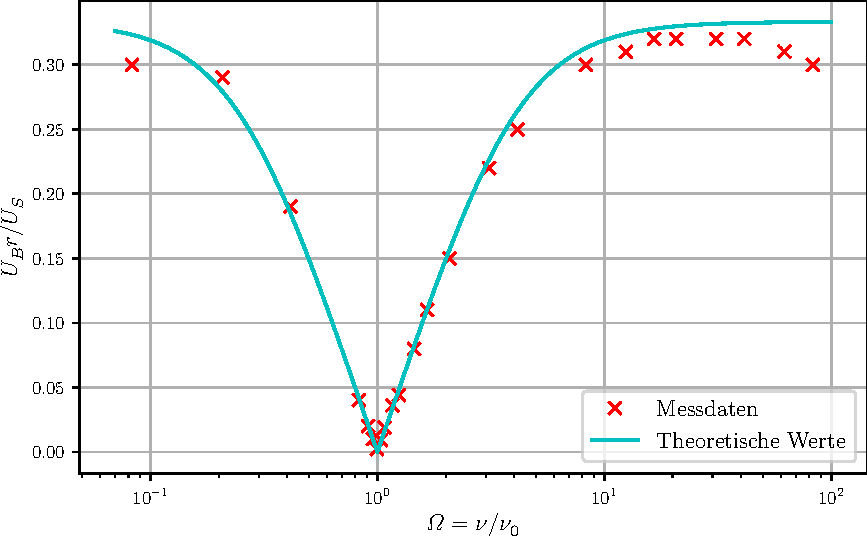
\includegraphics{plot.pdf}
  \caption{Plot.}
  \label{fig:plot}
\end{figure}


Siehe \autoref{fig:plot}!
